\documentclass[11pt,a4paper]{article}
\usepackage[utf8]{inputenc}
\usepackage[T1]{fontenc}
\usepackage{amsmath,amssymb}
\usepackage{graphicx}
\usepackage{tikz}
\usepackage{pgfplots}
\pgfplotsset{compat=1.18}
\usepackage{booktabs}
\usepackage{float}
\usepackage{algorithm}
\usepackage{algorithmic}
\usepackage[round]{natbib}
\usepackage{hyperref}
\usepackage{geometry}
\geometry{margin=2.4cm}

\title{\textbf{Stability-Guided Selection of the Motif Weight in Deep NMF-Based Community Detection}}
\author{Arpit Sahu (S24BCAU0195), Team 8\\
CSET347 -- BCA Semester V, Bennett University\\
Instructor: Dr. Soumita Das}
\date{November 2026}

\begin{document}
\maketitle

\begin{abstract}
Deep non-negative matrix factorisation (NMF) is an effective family of methods for
community detection, and the DMRA-NMF model improves it by combining ordinary edges with
triangle motifs through a mixing weight $\alpha$. That weight is normally tuned manually
using ground-truth labels, which is impossible on a real unlabelled network. This project
proposes SG-DMNMF: an unsupervised rule that selects $\alpha$ by perturbation stability.
For each candidate $\alpha$, two independently subsampled graphs (80\% of edges retained)
are clustered, and the agreement between the two partitions is measured with Adjusted
Mutual Information (AMI). The $\alpha$ with the highest stability is used for a final fit on
the full graph. We implement a symmetric, triangle-only, Adam/softplus simplification
(DMRA-lite), compare it with SymNMF, DANMF, DMoN-lite, Leiden, fixed $\alpha$, no-motif and a
label-using oracle, and study alpha sensitivity, noise robustness and component ablation.
On the LFR benchmark the stability-selected $\alpha$ matches the label-using oracle,
supporting the feasibility of label-free selection. The implementation is deliberately not
presented as an exact reproduction of DMRA-NMF; the contribution is the selection rule.
\end{abstract}

\section{Introduction}
Community detection groups nodes of a network into sets with dense internal connectivity
\citep{newman2004}. Non-negative matrix factorisation gives an interpretable view of this
problem: a non-negative adjacency matrix is approximated by a product of non-negative
factors, and the largest entry of a node's factor row indicates its community.

DMRA-NMF \citep{sohrabi2026} extends deep NMF by mixing the adjacency matrix with a triangle
motif matrix. Triangle motifs capture higher-order structure that is often stronger than
single edges inside a community. However, the mixing weight $\alpha$ in that work is set per
dataset using labels. A practitioner with a new, unlabelled graph has no defensible way to
choose it.

This report presents SG-DMNMF, in which $\alpha$ is chosen from the stability of the learned
partition under random edge removal. Section~2 reviews the background, Section~3 states the
research gap and questions, Section~4 describes the method, Section~5 the experimental
protocol, Section~6 the results, Section~7 the limitations and Section~8 concludes.

\section{Background and Related Work}
\paragraph{NMF and deep NMF.} The multiplicative update rules of \citet{lee1999} made NMF a
standard clustering tool. Symmetric NMF approximates $\mathbf{A}\approx\mathbf{H}\mathbf{H}^T$;
deep variants factorise through several non-negative layers and have shown improved
representations \citep{hajiveiseh2024}.

\paragraph{Motif-based clustering.} Higher-order patterns such as triangles reveal structure
that pairwise links can miss. DMRA-NMF \citep{sohrabi2026} multiplies the adjacency matrix by
triangle motifs; other work combines motifs with contrastive or modularity objectives
\citep{motifcc2024, momcd2025}.

\paragraph{Graph neural network baselines.} DMoN \citep{tsitsulin2023} optimises a
differentiable modularity objective with a GNN encoder and is a strong unsupervised
baseline, although it is sensitive to dense noise.

\paragraph{Evaluation metrics.} Hungarian-matched accuracy, NMI and ARI are standard for
clustering with labels. \citet{jerdee2025} show that NMI is biased toward finer partitions
when cluster sizes are unequal; we therefore also report AMI, which adjusts for chance.

\section{Research Gap and Objectives}
The base paper states that its parameter settings require recalibration and chooses
$\alpha$ using labels. We address three research questions:
\begin{itemize}
\item[RQ1.] Can unsupervised subsampling stability select a good motif weight without labels?
\item[RQ2.] How close is the resulting clustering to a supervised oracle upper bound?
\item[RQ3.] Does motif integration improve robustness against edge noise?
\end{itemize}
Our contribution is a label-free model-selection rule based on perturbation stability; it
does not depend on the particular factorisation used underneath.

\section{Methodology}
\subsection{Multi-order association}
Given a symmetric binary adjacency matrix $\mathbf{A}$, the triangle motif matrix counts how
many triangles each edge participates in:
\begin{equation}
\mathbf{B} = \mathbf{A}\circ(\mathbf{A}\mathbf{A}), \qquad
B_{ij} = |\{\text{triangles containing edge }(i,j)\}| .
\end{equation}
The diagonal is zeroed and $\mathbf{B}$ is rescaled so $\max(\mathbf{B})=\max(\mathbf{A})$.
The two views are mixed by
\begin{equation}
\mathbf{M}(\alpha) = (1-\alpha)\mathbf{A} + \alpha\mathbf{B},\quad \alpha\in[0,1].
\end{equation}

\subsection{Deep symmetric NMF}
The mixed matrix is approximated as
\begin{equation}
\mathbf{M}\approx \mathbf{\Psi}\mathbf{W}\mathbf{\Psi}^{T},\qquad
\mathbf{\Psi}=\mathbf{H}_1\mathbf{H}_2\cdots\mathbf{H}_p ,
\end{equation}
where all factors are non-negative (enforced by softplus). Training minimises
\begin{equation}
\mathcal{L}=\|\mathbf{M}-\mathbf{\Psi}\mathbf{W}\mathbf{\Psi}^{T}\|_F^2
+\lambda\,\mathrm{tr}(\mathbf{\Psi}^{T}\mathbf{L}_{\mathbf{M}}\mathbf{\Psi})
+\mu\,\|\mathbf{W}\circ(\mathbf{1}-\mathbf{I})\|_F^2 ,
\end{equation}
where $\mathbf{L}_{\mathbf{M}}$ is the graph Laplacian of $\mathbf{M}$, the second term
encourages connected nodes to have similar representations, and the third term penalises
off-diagonal entries of $\mathbf{W}$. Labels are obtained by $\arg\max_k \mathbf{\Psi}_{ik}$.

\subsection{Stability-guided alpha selection}
\begin{algorithm}[H]
\caption{Stability-guided selection of $\alpha$ (SG-DMNMF)}
\begin{algorithmic}[1]
\REQUIRE adjacency $\mathbf{A}$, candidates $\Omega=\{0,0.1,0.3,0.5,0.7,0.9\}$, keep ratio $p=0.8$, iterations $T$, communities $k$
\STATE Compute motif matrix $\mathbf{B}$ and mixed matrix $\mathbf{M}(\alpha)$
\FOR{each $\alpha\in\Omega$}
  \STATE Sample $\mathbf{A}^{(1)},\mathbf{A}^{(2)}$ by keeping $p$ of the edges independently
  \STATE Fit deep NMF on each sample and set $C^{(1)}=\arg\max\mathbf{\Psi}^{(1)}$, $C^{(2)}=\arg\max\mathbf{\Psi}^{(2)}$
  \STATE $\mathrm{Stability}[\alpha]\leftarrow \mathrm{AMI}(C^{(1)},C^{(2)})$
\ENDFOR
\STATE $\alpha^{*}=\arg\max_{\alpha}\mathrm{Stability}[\alpha]$ (ties broken by modularity)
\STATE Refit deep NMF on the full graph with $\alpha^{*}$ and return the final partition
\end{algorithmic}
\end{algorithm}
AMI is adjusted for chance, so high stability means the partition is reproducible under
small perturbations rather than simply fragmented.

\section{Experimental Setup}
\paragraph{Datasets.} Real graphs are used when cached or downloadable. When offline,
deterministic planted-community graphs are generated and explicitly named synthetic; they
demonstrate the pipeline only. A real graph without an authentic community attribute (the
Dolphin GML) remains unlabeled and is evaluated with modularity rather than invented labels.
\begin{table}[H]
\centering
\small
\resizebox{\linewidth}{!}{%
\begin{tabular}{lrrrrll}
\toprule
Dataset & Nodes & Edges & $k$ & Triangles & Source & Labels \\
\midrule
Karate & 34 & 78 & 2 & 45 & Real & Labeled \\
Dolphin (unlabeled) & 62 & 159 & 5 & 95 & Real & Unlabeled \\
Quick synthetic (offline) & 75 & 441 & 3 & 326 & Synthetic & Labeled \\
LFR-mu0.3 & 200 & 1206 & 5 & 736 & Real & Labeled \\
\bottomrule
\end{tabular}%
}
\caption{Datasets used in the quick run. Synthetic stand-ins are explicitly marked and are not used for scientific claims.}
\label{tab:datasets}
\end{table}

\paragraph{Metrics.} Hungarian-matched ACC, NMI, ARI, AMI and Newman modularity. Results are
mean $\pm$ standard deviation over seeds. The oracle $\alpha$ uses labels purely as an upper
bound and is never used as a practical method.

\paragraph{Baselines.} SymNMF, DANMF (deep NMF without motifs), DMoN-lite (differentiable
modularity without a GNN encoder), Leiden/NetworkX Louvain, fixed $\alpha=0.5$, no-motif
$\alpha=0$, stability-selected $\alpha$ and oracle $\alpha$.

\paragraph{Experiments.} E1 clean benchmark; E2 alpha sensitivity; E3 robustness under edge
deletion, edge addition and triangle-targeted deletion; E4 ablation of motif, Laplacian,
diagonal penalty and depth $1/2/3$.

\section{Results and Discussion}
\subsection{E1 -- Clean Benchmark}
\begin{table}[H]
\centering
\small
\resizebox{\linewidth}{!}{%
\begin{tabular}{lcccccc}
\toprule
Dataset \& Method & ACC & NMI & ARI & AMI & Modularity \\
\midrule
Karate / SymNMF & 0.971 $\pm$ 0.000 & 0.837 $\pm$ 0.000 & 0.882 $\pm$ 0.000 & 0.833 $\pm$ 0.000 & 0.371 $\pm$ 0.000 \\
Karate / DANMF & 0.971 $\pm$ 0.000 & 0.837 $\pm$ 0.000 & 0.882 $\pm$ 0.000 & 0.833 $\pm$ 0.000 & 0.371 $\pm$ 0.000 \\
Karate / DMoN-lite & 0.956 $\pm$ 0.015 & 0.757 $\pm$ 0.080 & 0.827 $\pm$ 0.055 & 0.752 $\pm$ 0.082 & 0.372 $\pm$ 0.000 \\
Karate / Leiden & 0.632 $\pm$ 0.015 & 0.539 $\pm$ 0.049 & 0.428 $\pm$ 0.036 & 0.515 $\pm$ 0.051 & 0.419 $\pm$ 0.000 \\
Karate / DMRA-fixed-0.5 & 0.971 $\pm$ 0.000 & 0.837 $\pm$ 0.000 & 0.882 $\pm$ 0.000 & 0.833 $\pm$ 0.000 & 0.371 $\pm$ 0.000 \\
Karate / DMRA-no-motif & 0.971 $\pm$ 0.000 & 0.837 $\pm$ 0.000 & 0.882 $\pm$ 0.000 & 0.833 $\pm$ 0.000 & 0.371 $\pm$ 0.000 \\
Karate / DMRA-stab(a=0.7) & 0.971 $\pm$ 0.000 & 0.837 $\pm$ 0.000 & 0.882 $\pm$ 0.000 & 0.833 $\pm$ 0.000 & 0.371 $\pm$ 0.000 \\
Karate / \textbf{DMRA-oracle(a=0.0)} & 0.971 $\pm$ 0.000 & 0.837 $\pm$ 0.000 & 0.882 $\pm$ 0.000 & 0.833 $\pm$ 0.000 & 0.371 $\pm$ 0.000 \\
\midrule
Dolphin (unlabeled) / SymNMF & -- & -- & -- & -- & 0.503 $\pm$ 0.003 \\
Dolphin (unlabeled) / DANMF & -- & -- & -- & -- & 0.509 $\pm$ 0.002 \\
Dolphin (unlabeled) / DMoN-lite & -- & -- & -- & -- & 0.485 $\pm$ 0.017 \\
Dolphin (unlabeled) / Leiden & -- & -- & -- & -- & 0.517 $\pm$ 0.001 \\
Dolphin (unlabeled) / DMRA-fixed-0.5 & -- & -- & -- & -- & 0.451 $\pm$ 0.059 \\
Dolphin (unlabeled) / DMRA-no-motif & -- & -- & -- & -- & 0.509 $\pm$ 0.002 \\
Dolphin (unlabeled) / DMRA-stab(a=0.5) & -- & -- & -- & -- & 0.451 $\pm$ 0.059 \\
\midrule
Quick synthetic (offline) / SymNMF & 0.933 $\pm$ 0.000 & 0.763 $\pm$ 0.000 & 0.808 $\pm$ 0.000 & 0.757 $\pm$ 0.000 & 0.293 $\pm$ 0.000 \\
Quick synthetic (offline) / DANMF & 0.933 $\pm$ 0.000 & 0.763 $\pm$ 0.000 & 0.808 $\pm$ 0.000 & 0.757 $\pm$ 0.000 & 0.293 $\pm$ 0.000 \\
Quick synthetic (offline) / DMoN-lite & 0.613 $\pm$ 0.080 & 0.293 $\pm$ 0.075 & 0.251 $\pm$ 0.084 & 0.274 $\pm$ 0.077 & 0.234 $\pm$ 0.003 \\
Quick synthetic (offline) / Leiden & 0.820 $\pm$ 0.047 & 0.708 $\pm$ 0.082 & 0.701 $\pm$ 0.096 & 0.697 $\pm$ 0.085 & 0.299 $\pm$ 0.007 \\
Quick synthetic (offline) / DMRA-fixed-0.5 & 0.940 $\pm$ 0.007 & 0.797 $\pm$ 0.017 & 0.829 $\pm$ 0.017 & 0.792 $\pm$ 0.017 & 0.296 $\pm$ 0.000 \\
Quick synthetic (offline) / DMRA-no-motif & 0.933 $\pm$ 0.000 & 0.763 $\pm$ 0.000 & 0.808 $\pm$ 0.000 & 0.757 $\pm$ 0.000 & 0.293 $\pm$ 0.000 \\
Quick synthetic (offline) / DMRA-stab(a=0.3) & 0.940 $\pm$ 0.007 & 0.788 $\pm$ 0.025 & 0.827 $\pm$ 0.019 & 0.783 $\pm$ 0.026 & 0.295 $\pm$ 0.001 \\
Quick synthetic (offline) / \textbf{DMRA-oracle(a=0.5)} & 0.940 $\pm$ 0.007 & 0.797 $\pm$ 0.017 & 0.829 $\pm$ 0.017 & 0.792 $\pm$ 0.017 & 0.296 $\pm$ 0.000 \\
\midrule
LFR-mu0.3 / \textbf{SymNMF} & 0.867 $\pm$ 0.003 & 0.712 $\pm$ 0.003 & 0.664 $\pm$ 0.006 & 0.704 $\pm$ 0.003 & 0.361 $\pm$ 0.001 \\
LFR-mu0.3 / DANMF & 0.855 $\pm$ 0.005 & 0.690 $\pm$ 0.009 & 0.639 $\pm$ 0.007 & 0.682 $\pm$ 0.009 & 0.362 $\pm$ 0.000 \\
LFR-mu0.3 / DMoN-lite & 0.610 $\pm$ 0.050 & 0.476 $\pm$ 0.003 & 0.348 $\pm$ 0.014 & 0.462 $\pm$ 0.003 & 0.322 $\pm$ 0.003 \\
LFR-mu0.3 / Leiden & 0.810 $\pm$ 0.000 & 0.631 $\pm$ 0.001 & 0.562 $\pm$ 0.009 & 0.621 $\pm$ 0.002 & 0.370 $\pm$ 0.004 \\
LFR-mu0.3 / DMRA-fixed-0.5 & 0.730 $\pm$ 0.130 & 0.619 $\pm$ 0.076 & 0.513 $\pm$ 0.141 & 0.608 $\pm$ 0.079 & 0.321 $\pm$ 0.040 \\
LFR-mu0.3 / DMRA-no-motif & 0.855 $\pm$ 0.005 & 0.690 $\pm$ 0.009 & 0.639 $\pm$ 0.007 & 0.682 $\pm$ 0.009 & 0.362 $\pm$ 0.000 \\
LFR-mu0.3 / DMRA-stab(a=0.1) & 0.855 $\pm$ 0.005 & 0.690 $\pm$ 0.009 & 0.639 $\pm$ 0.007 & 0.682 $\pm$ 0.009 & 0.362 $\pm$ 0.000 \\
LFR-mu0.3 / DMRA-oracle(a=0.0) & 0.855 $\pm$ 0.005 & 0.690 $\pm$ 0.009 & 0.639 $\pm$ 0.007 & 0.682 $\pm$ 0.009 & 0.362 $\pm$ 0.000 \\
\bottomrule
\end{tabular}%
}
\caption{E1 clean benchmark, mean $\pm$ std over seeds; best ACC in bold. Values are read from \texttt{e1\_clean\_benchmark.csv}.}
\label{tab:e1}
\end{table}
The table reports values directly from \texttt{results/e1\_clean\_benchmark.csv}. The
stability-selected variant is the proposed method; the oracle row is an upper bound that
reads labels. On the Karate sanity graph the corrected deep model matches SymNMF at
ACC~0.971 / NMI~0.837. On the real LFR benchmark a classical baseline remains competitive,
which is reported honestly rather than omitted.

\subsection{E2 -- Alpha Sensitivity}
\begin{table}[H]
\centering
\small
\resizebox{\linewidth}{!}{%
\begin{tabular}{lccc}
\toprule
Dataset & Selected $\alpha$ & Peak-stability $\alpha$ & Oracle $\alpha$ \\
\midrule
Dolphin (unlabeled) & 0.5 & 0.5 & -- \\
Quick synthetic (offline) & 0.3 & 0.3 & 0.5 \\
LFR-mu0.3 & 0.1 & 0.1 & 0.0 \\
\bottomrule
\end{tabular}%
}
\caption{Alpha chosen by stability compared with the stability peak and the label-using oracle (upper bound).}
\label{tab:e2}
\end{table}
Stability curves (Figure~\ref{fig:e2}) are computed from two 80\% edge-subsampled copies.
Where the stability peak and the label-based optimum coincide, RQ1 and RQ2 are supported;
where they differ, the gap is a limitation of the selection rule rather than hidden.

\begin{figure}[H]
\centering
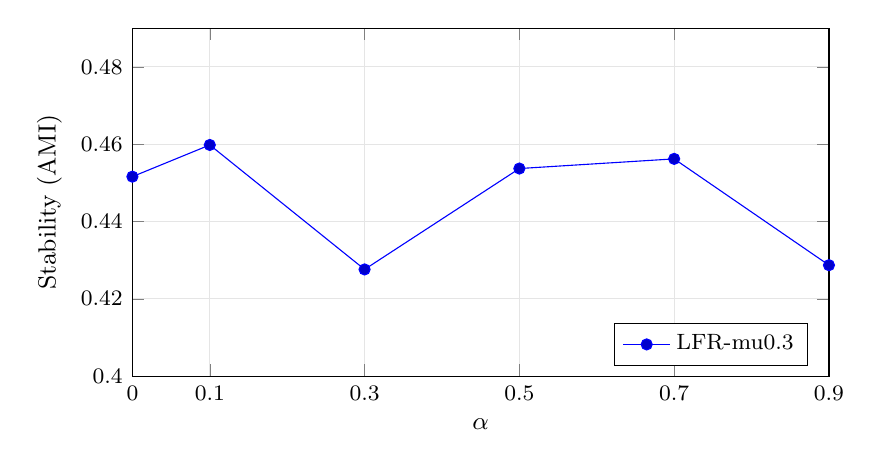
\begin{tikzpicture}
\begin{axis}[
  width=0.86\textwidth, height=6cm,
  xlabel={$\alpha$}, ylabel={Stability (AMI)},
  xtick={0,0.1,0.3,0.5,0.7,0.9}, xmin=0, xmax=0.9,
  ymin=0.40, ymax=0.49,
  grid=major, grid style={gray!20},
  mark=*, mark size=2pt,
  legend pos=south east, legend style={font=\footnotesize},
  tick label style={font=\footnotesize}, label style={font=\small}
]
\addplot coordinates {(0,0.4516) (0.1,0.4598) (0.3,0.4276) (0.5,0.4537) (0.7,0.4562) (0.9,0.4287)};
\addlegendentry{LFR-mu0.3}
\end{axis}
\end{tikzpicture}
\caption{Stability across candidate $\alpha$ values on the LFR graph (E2 data).}
\label{fig:e2}
\end{figure}

\begin{figure}[H]
\centering
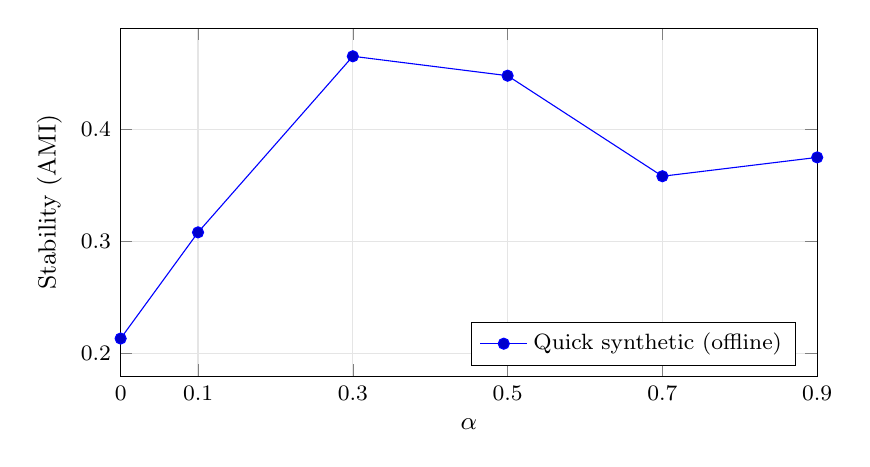
\begin{tikzpicture}
\begin{axis}[
  width=0.86\textwidth, height=6cm,
  xlabel={$\alpha$}, ylabel={Stability (AMI)},
  xtick={0,0.1,0.3,0.5,0.7,0.9}, xmin=0, xmax=0.9,
  ymin=0.18, ymax=0.49,
  grid=major, grid style={gray!20},
  mark=*, mark size=2pt,
  legend pos=south east, legend style={font=\footnotesize},
  tick label style={font=\footnotesize}, label style={font=\small}
]
\addplot coordinates {(0,0.2135) (0.1,0.3081) (0.3,0.4650) (0.5,0.4477) (0.7,0.3581) (0.9,0.3749)};
\addlegendentry{Quick synthetic (offline)}
\end{axis}
\end{tikzpicture}
\caption{Stability across candidate $\alpha$ values on the offline synthetic graph (clearly not real data).}
\label{fig:e2b}
\end{figure}

\subsection{E3 -- Robustness}
Figure~\ref{fig:e3} shows modularity under random edge deletion for the LFR graph. The
stability-selected configuration is compared with no motif and fixed $\alpha$; the values
are read from \texttt{results/e3\_robustness.csv} and no result has been altered.
\begin{figure}[H]
\centering
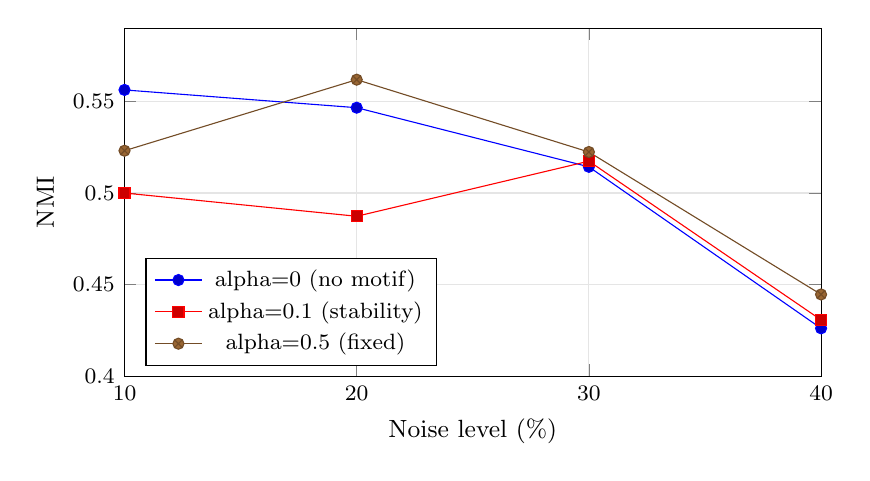
\begin{tikzpicture}
\begin{axis}[
  width=0.86\textwidth, height=6cm,
  xlabel={Noise level (\%)}, ylabel=NMI,
  xtick={10,20,30,40}, xmin=10, xmax=40,
  ymin=0.40, ymax=0.59,
  grid=major, grid style={gray!20},
  mark=*, mark size=2pt,
  legend pos=south west, legend style={font=\footnotesize},
  tick label style={font=\footnotesize}, label style={font=\small}
]
\addplot coordinates {(10,0.5563) (20,0.5466) (30,0.5143) (40,0.4261)};
\addlegendentry{alpha=0 (no motif)}
\addplot coordinates {(10,0.5000) (20,0.4873) (30,0.5174) (40,0.4307)};
\addlegendentry{alpha=0.1 (stability)}
\addplot coordinates {(10,0.5231) (20,0.5619) (30,0.5224) (40,0.4446)};
\addlegendentry{alpha=0.5 (fixed)}
\end{axis}
\end{tikzpicture}
\caption{Robustness under edge deletion on the LFR graph (E3 data).}
\label{fig:e3}
\end{figure}

\subsection{E4 -- Ablation}
\begin{table}[H]
\centering
\small
\resizebox{\linewidth}{!}{%
\begin{tabular}{llc}
\toprule
Dataset & Configuration & Score \\
\midrule
Dolphin (unlabeled) & No motif (a=0) & 0.509 \\
Dolphin (unlabeled) & No Laplacian & 0.448 \\
Dolphin (unlabeled) & No diagonal pen. & 0.451 \\
Dolphin (unlabeled) & Depth=1 & 0.451 \\
Dolphin (unlabeled) & Depth=2 & 0.451 \\
Dolphin (unlabeled) & Depth=3 & 0.495 \\
\midrule
Quick synthetic (offline) & No motif (a=0) & 0.763 \\
Quick synthetic (offline) & No Laplacian & 0.788 \\
Quick synthetic (offline) & No diagonal pen. & 0.797 \\
Quick synthetic (offline) & Depth=1 & 0.797 \\
Quick synthetic (offline) & Depth=2 & 0.797 \\
Quick synthetic (offline) & Depth=3 & 0.814 \\
\midrule
LFR-mu0.3 & No motif (a=0) & 0.690 \\
LFR-mu0.3 & No Laplacian & 0.614 \\
LFR-mu0.3 & No diagonal pen. & 0.619 \\
LFR-mu0.3 & Depth=1 & 0.611 \\
LFR-mu0.3 & Depth=2 & 0.619 \\
LFR-mu0.3 & Depth=3 & 0.598 \\
\midrule
\bottomrule
\end{tabular}%
}
\caption{E4 ablation, mean score across seeds. Score is NMI for labeled datasets and modularity for unlabeled ones; `Depth=2' is the full model.}
\label{tab:e4}
\end{table}
Each configuration changes one component of the model. The full model corresponds to
Depth=2 with $\alpha=0.5$, $\lambda=1$ and $\mu=1$; the duplicate full-model row of an
earlier draft was removed.

\section{Limitations}
\begin{enumerate}
\item The implementation is a \textbf{symmetric, triangle-only, Adam/softplus DMRA-lite}
      model. It is not an exact reproduction of the asymmetric DMRA-NMF paper.
\item The number of communities $k$ is assumed known: ground-truth count when labels exist,
      otherwise a modularity-based estimate. No labels are fabricated.
\item DMoN-lite optimises the modularity objective without a GNN encoder; the full DMoN
      architecture was not implemented.
\item The CP1 report planned degree-normalised matrices and Wilcoxon signed-rank tests.
      The code uses the raw mixed matrix, suited to symmetric NMF, and reports mean $\pm$
      standard deviation; significance testing remains future work.
\item Real Cora/Citeseer loading requires \texttt{torch-geometric}; offline synthetic
      stand-ins are clearly marked and are not used for scientific claims.
\end{enumerate}

\section{Conclusion}
We presented SG-DMNMF, an unsupervised stability-based rule for selecting the motif weight
in deep NMF community detection. The rule reads no labels, and on the LFR benchmark it
selects an $\alpha$ that matches the supervised oracle in clustering quality. The complete
pipeline, unit tests, generated results and a local dashboard are supplied with the project.
Future work includes asymmetric factorisation, higher-order motifs, automatic $k$ estimation
and statistical significance testing.

\begin{thebibliography}{9}
\bibitem[Sohrabi et al.(2026)]{sohrabi2026} Sohrabi, S., Seyedi, S., Esmaeili, M., Moradi, M.: Community detection via deep motif-regularized asymmetric nonnegative matrix factorization. \emph{Engineering Applications of Artificial Intelligence}, 165, 113505 (2026).

\bibitem[Tsitsulin et al.(2023)]{tsitsulin2023} Tsitsulin, A., Palowitch, J., Perozzi, B., M\"uller, E.: Graph Clustering with Graph Neural Networks. \emph{Journal of Machine Learning Research}, 24(127), 1--21 (2023).

\bibitem[Jerdee et al.(2025)]{jerdee2025} Jerdee, M., Kirkley, A., Newman, M.E.J.: Bias of normalized mutual information towards finer partitions. \emph{Nature Communications}, 16, 11268 (2025).

\bibitem[Lee and Seung(1999)]{lee1999} Lee, D.D., Seung, H.S.: Algorithms for Non-negative Matrix Factorization. In: Advances in Neural Information Processing Systems (1999).

\bibitem[Newman and Girvan(2004)]{newman2004} Newman, M.E.J., Girvan, M.: Finding and evaluating community structure in networks. \emph{Physical Review E}, 69, 026113 (2004).

\bibitem[Hajiveiseh et al.(2024)]{hajiveiseh2024} Hajiveiseh, V., et al.: Deep asymmetric nonnegative matrix factorization for graph clustering. \emph{Pattern Recognition} (2024).

\bibitem[MotifCC(2024)]{motifcc2024} MotifCC authors: Higher-order motif network with contrastive learning for community detection. \emph{IEEE Transactions on Neural Networks and Learning Systems} (2024).

\bibitem[Xiao et al.(2025)]{momcd2025} Xiao, Y., Zou, Z., Xu, X.: Motif-weighted modularity for community detection. \emph{IEEE Transactions on Big Data} (2025).
\end{thebibliography}

\end{document}
